   \documentclass{beamer}
%
% Choose how your presentation looks.
%
% For more themes, color themes and font themes, see:
% http://deic.uab.es/~iblanes/beamer_gallery/index_by_theme.html
%
\mode<presentation>
{
  \usetheme{Boadilla}     % or try Boadilla, Darmstadt, Madrid, Warsaw, default, ...
  \usecolortheme{default} % or try Boadilla, albatross, beaver, crane, default, ...
  \usefonttheme{default}  % or try Boadilla, serif, structurebold, default, ...
  \setbeamertemplate{navigation symbols}{}
  \setbeamertemplate{caption}[numbered]
} 

\usepackage[english]{babel}
\usepackage[utf8x]{inputenc}
\usepackage{caption}
\usepackage{subcaption}
\newenvironment{variableblock}[3]{%
  \setbeamercolor{block body}{#2}
  \setbeamercolor{block title}{#3}
  \begin{block}{#1}}{\end{block}}
\title[Software Colaborativo lantonistas]{Optical Isolation with Nonlinear Topological Photonics}
%\author[CDTec] {Cristian Pereira, André Einhardt, Mateus Nascimento}
\author[CDTec] {Xin Zhou, You Wang, Daniel Leykam and Yidong Chong}

\institute[]{Nanyang Technological University, Singapore}
\date{September 2017}


\begin{document}

\begin{frame}
    \begin{center}
  \titlepage 
      \begin{figure}[h]
  
\includegraphics[width=2.3cm,height=2.3cm] {/home/zhouxin/research/conference/presentation/mtheme/slides/icon.png}
  
\includegraphics[width=3.5cm,height=2.1cm,scale=1] {/home/zhouxin/research/conference/presentation/mtheme/slides/icon.png}
      \end{figure}
  \end{center}
\end{frame}

% Uncomment these lines for an automatically generated outline.
%\begin{frame}{Outline}
%  \tableofcontents
%\end{frame}

\section{Outline}
\begin{frame}{Outline}
    \begin{itemize}
      \item Optical Isolation
      \begin{itemize}
      \item What is optical isolator
      \item Why we want optical isolator
      \item How to achieve optical isolation
      \end{itemize}
      \item Topological Photonics
            \begin{itemize}
            \item Topological state
            \item Realizing Topological Edge State in Photonic System
		    \end{itemize}
      
      \item Topological Optical Isolation 
            \begin{itemize}
            \item 1D SSH model
            \item 2D Haldane model
            \item 2D lattice of coupled ring waveguides
		    \end{itemize}
	  \end{itemize}        
  \vskip 5cm
\end{frame}

\section{Optical Isolation}
% ================== ÁREAS SENDO ALTERADAS POR CRISTIAN PEREIRA ==================
\begin{frame}{What is Optical Isolation}
Optical isolators are devices that allow light to pass in one direction (e.g., along a waveguide), while blocking transmission in the other direction, thus acting as the analogues of diodes in electronic circuits
\begin{itemize}
    \item Facilita
\end{itemize}
\vskip 3cm
\end{frame}

\begin{frame}{Why We Need Optical Isolator}
    \begin{block}
    {Reason}
      \begin{itemize}
        \item In modern fibre communication networks it is an essential device to prevent interference between different parts of the networks.
    \end{itemize}
  \end{block}
  \vskip 1cm
  \begin{block}{Why need on-chip size optical isolator}
    \begin{itemize}
        \item Nowadays people become more and more interested in large-scale on-chip networks, so optical isolation on-chip size is becoming increasingly important. 
    \end{itemize}
  \end{block}
\end{frame}



\begin{frame}{How to Achieve Optical Isolation}
    \begin{block}{Lorenz Reciprocity}

For linear, static and non-magnetic material,
     \vskip -0.75cm
\begin{equation}
\nabla \cdot (\textbf{$E^{'}$} \times\textbf{$H^{''}$} - \textbf{$E^{''}$} \times\textbf{$H^{'}$}) = j\omega(\textbf{$E^{''}$} \textbf{$\epsilon$} \textbf{$E^{'}$} - \textbf{$E^{'}$} \textbf{$\epsilon$} \textbf{$E^{''}$} - H^{''} \mu \textbf{$H^{'}$}+H^{'} \mu \textbf{$H^{''}$} ) = 0 
\end{equation}
     \vskip -0.25cm
Here, ($E^{'}, H^{'}$) and ($E^{''}, H^{''}$) are two sets of excitation.
  \end{block}
  


  
\textbf{Ways to break Lorenz Reciprocity}
    \begin{block}{Magneto-Optical Effect}
For magneto-optical material so $\epsilon$ and $\mu$ are non-symmetric tensor.
  \end{block}
%  \vskip -1cm
  \begin{block}{Optical Nonlinearity}
For nonlinear material, right side of Eq.(1) = $j\omega(\textbf{$E^{''}$} \textbf{$\epsilon$}(E^{'}) \textbf{$E^{'}$} - \textbf{$E^{'}$} \textbf{$\epsilon$}(E^{''}) \textbf{$E^{''}$} - H^{''} \mu(H^{'}) \textbf{$H^{'}$}+H^{'} \mu(H^{''}) \textbf{$H^{''}$} )$
  \end{block}
%  \vskip 1cm
  \begin{block}{Spacial-temporal Modulation}
 For $\epsilon$ and $\mu$ depend on time, the derivation is not valid, so does Lorentz Reciprocity.
  \end{block}
\end{frame}

\begin{frame}{How to Achieve Optical solation}
     \vskip -0.15cm
    \begin{block}{Lorenz Reciprocity}

For linear, static and non-magnetic material,
     \vskip -0.75cm
\begin{equation}
\nabla \cdot (\textbf{$E^{'}$} \times\textbf{$H^{''}$} - \textbf{$E^{''}$} \times\textbf{$H^{'}$}) = j\omega(\textbf{$E^{''}$} \textbf{$\epsilon$} \textbf{$E^{'}$} - \textbf{$E^{'}$} \textbf{$\epsilon$} \textbf{$E^{''}$} - H^{''} \mu \textbf{$H^{'}$}+H^{'} \mu \textbf{$H^{''}$} ) = 0 
\end{equation}
     \vskip -0.25cm
Here, ($E^{'}, H^{'}$) and ($E^{''}, H^{''}$) are two sets of excitation.
  \end{block}
       \vskip -0.75cm
\begin{columns}[t]
  \begin{column}{0.325\textwidth}
    \begin{block}{Magneto-Optical Effect}
For magneto-optical material so $\epsilon$ and $\mu$ are non-symmetric tensor.
     \vskip -0.4cm
  \begin{figure}
    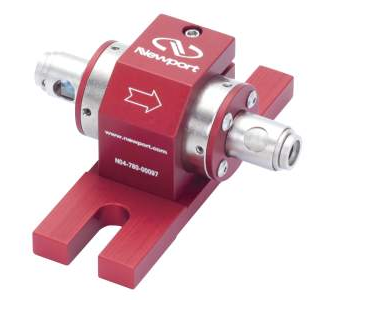
\includegraphics[width=3cm,height=2cm] {/home/zhouxin/research/conference/presentation/mtheme/slides/isolator_faraday.png}
         \vskip -0.4cm
    \caption{Commercial Faraday Optical Isolator}
  \end{figure}
    \end{block}
  \end{column}
  \begin{column}{0.325\textwidth}
    \begin{block}{Optical Nonlinear Material}
      For nonlinear material,$\epsilon$ and $\mu$ depend on $E$ and $H$
   \vskip -0.85cm
  \begin{figure}
\captionsetup{font=small,labelfont=small}
    \includegraphics[width=4cm,height=2.5cm] {/home/zhouxin/research/conference/presentation/mtheme/slides/pt_isolator.pdf}
         \vskip -0.4cm
     \end{figure}
{
\tiny Peng, Bo, et al Nature Physics 10.5 (2014): 394} 
    \end{block}
  \end{column}
  \begin{column}{0.325\textwidth}
    \begin{block}{Spacial-temporal Modulation}
      For $\epsilon$ and $\mu$ depend on time, the derivation is not valid, so does Lorentz Reciprocity.
    \end{block}
  \end{column}

\end{columns}
\end{frame}

\begin{frame}{Topological Photonics}
\begin{block}{Discover of Topological State}
Insulating in the bulk while conducting in the surface without backscattering even in the presence of impurities.
\begin{figure}
    \centering
    \begin{subfigure}[t]{0.4\textwidth}
        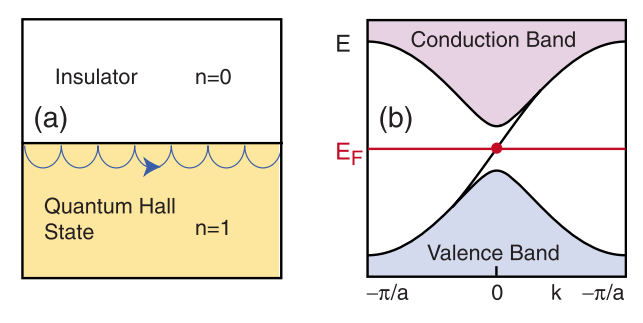
\includegraphics[width=\textwidth]{/home/zhouxin/research/conference/presentation/mtheme/slides/hall.png}
        \caption{Quantum Hall Effect. Time reversal symmetry is broken. Hasan and Kane, RMP, 2010}
        \label{fig:gull}
    \end{subfigure}\hspace*{3.0em}%
    ~ %add desired spacing between images, e. g. ~, \quad, \qquad, \hfill etc. 
      %(or a blank line to force the subfigure onto a new line)
    \begin{subfigure}[t]{0.415\textwidth}
        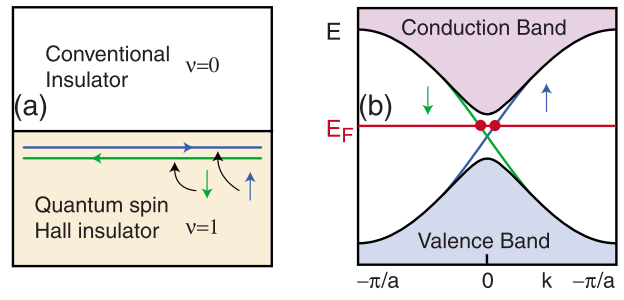
\includegraphics[width=\textwidth]{/home/zhouxin/research/conference/presentation/mtheme/slides/spin_hall.png}
        \caption{Quantum Spin Hall Effect. Time reversal symmetry is preserved. Hasan and Kane, RMP, 2010}
        \label{fig:tiger}
    \end{subfigure}
\label{fig:animals}
\end{figure}      

%\begin{variableblock}{Title}{bg=white}{bg=white}
%d
%\end{variableblock}

\end{block}

\end{frame}
\begin{frame}{Topological Photonics}
\begin{block}{Realize Topological State in Photonic System}

\begin{figure}
    \centering
    \begin{subfigure}[t]{0.4\textwidth}
        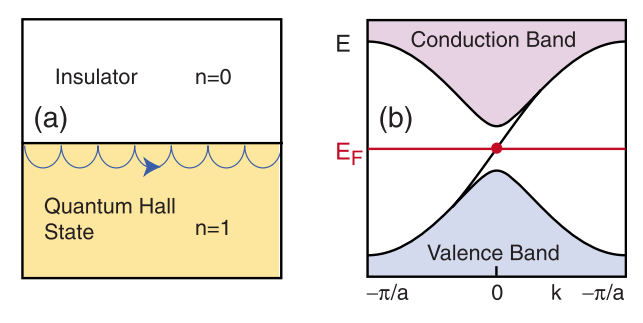
\includegraphics[width=\textwidth]{/home/zhouxin/research/conference/presentation/mtheme/slides/hall.png}
        \caption{Quantum Hall Effect. Time reversal symmetry is broken. Hasan and Kane, RMP, 2010}
        \label{fig:gull}
    \end{subfigure}\hspace*{3.0em}%
    ~ %add desired spacing between images, e. g. ~, \quad, \qquad, \hfill etc. 
      %(or a blank line to force the subfigure onto a new line)
    \begin{subfigure}[t]{0.415\textwidth}
        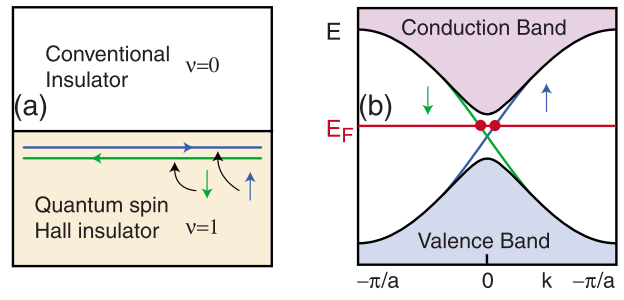
\includegraphics[width=\textwidth]{/home/zhouxin/research/conference/presentation/mtheme/slides/spin_hall.png}
        \caption{Quantum Spin Hall Effect. Time reversal symmetry is preserved. Hasan and Kane, RMP, 2010}
        \label{fig:tiger}
    \end{subfigure}
\label{fig:animals}
\end{figure}      

%\begin{variableblock}{Title}{bg=white}{bg=white}
%d
%\end{variableblock}

\end{block}

\end{frame}
% =================================== FIM MATEUS =================================
\end{document}
